% =====================================================================
%  SchemaLens no Apache Cassandra: metodologia e avaliacao em quatro benchmarks
%  (IoT-Benchmark, TPCx-IoT, TSBS e RUBiS) sob um protocolo comum de execucao.
%  Compilar no Overleaf com pdfLaTeX. Tabelas em tables/ geradas por build_tables.py.
% =====================================================================
\documentclass[10pt,a4paper,twoside]{article}
\usepackage[T1]{fontenc}
\usepackage[utf8]{inputenc}
\usepackage{lmodern}
\IfFileExists{brazil.ldf}{\usepackage[brazil]{babel}}{}
\usepackage[a4paper,margin=2.0cm]{geometry}
\usepackage{amsmath,amssymb,amsthm}
\usepackage{graphicx,booktabs,tabularx,longtable,array,float}
\usepackage[font=small,labelfont=bf]{caption}
\usepackage[table]{xcolor}
\usepackage{microtype}
\IfFileExists{enumitem.sty}{\usepackage{enumitem}\setlist{itemsep=1pt,topsep=2pt}}{}
\usepackage[colorlinks=true,linkcolor=blue!50!black,urlcolor=blue!50!black,citecolor=green!40!black]{hyperref}
\emergencystretch=3em
\newcolumntype{Y}{>{\raggedright\arraybackslash}X}
\makeatletter\newcommand{\tabin}[1]{\@@input #1 }\makeatother
\definecolor{boxbg}{RGB}{243,246,250}
\newcommand{\caixa}[1]{\par\smallskip\noindent\colorbox{boxbg}{\parbox{\dimexpr\linewidth-2\fboxsep}{#1}}\par\smallskip}
\theoremstyle{definition}\newtheorem{definicao}{Definição}

\title{\textbf{SchemaLens no Apache Cassandra}\\[3pt]
\large Redução explicável do espaço de projetos físicos e sua avaliação em três benchmarks de séries temporais e no RUBiS, sob um protocolo comum de execução}
\author{Projeto SchemaLens / Cassandra}
\date{Versão ajustada --- novembro de 2026}

\begin{document}
\maketitle

\begin{abstract}
\noindent O SchemaLens gera, \emph{antes de qualquer medição}, um conjunto pequeno e explicável de projetos físicos candidatos (HBench) a partir de evidências do workload. Ele ativa famílias de estruturas por regras declarativas, instancia candidatos, sintetiza rotas de leitura e escrita, estima custos analíticos e seleciona configurações completas. Este artigo descreve a metodologia aplicada ao Apache Cassandra e a avalia em quatro benchmarks: três de séries temporais (IoT-Benchmark, TPCx-IoT e TSBS cpu-only) e o RUBiS. Uma análise de consistência entre os experimentos mostrou que a fase de projeto já era comum, mas que a fase de medição divergia em versão do Cassandra, métrica, estatística, controle de estado físico, avaliação de preservação e ablações. Por isso definimos e congelamos um \textbf{protocolo comum de execução (v1)} e reexecutamos a medição dos quatro benchmarks sob ele:
\begin{itemize}
\item imagem fixada por digest, em container dedicado;
\item 5 repetições com reinício a frio e gate de flush;
\item ordem contrabalançada;
\item oráculo independente em todas as respostas;
\item média, p50, p95 e p99, com IC por bootstrap e piso de ruído por réplicas A/A;
\item Top-$k$, regret, retenção de Pareto e ablações;
\item gates de aceitação recalculados dos dados brutos.
\end{itemize}
Nos três TSDB, o HBench preservou o melhor deployment medido, com regret de 0 a 0,2\% e redução do espaço de 44\% a 50\%. O escore analítico, porém, só ordena bem a latência quando o espaço tem diferenças estruturais grandes. Os resultados diante das referências variam por benchmark: empate com o desenho de referência no IoT (mesmo DDL), empate em leitura e perda em escrita diante do baseline TPCx, e ganho de 1,7$\times$ sobre o esquema original do TSBS. No RUBiS, medido com os mesmos dados em Cassandra 4.1.12 e 3.11.11, as conclusões centrais da versão anterior se mantêm: H01 é 25 a 36\% mais rápido que NoSE e QPG nas cargas de leitura e mistas. Também quantificamos que a versão do Cassandra, sozinha, altera as latências absolutas em 14 a 38\%.
\end{abstract}

\tableofcontents
\newpage

% =====================================================================
\section{Introdução}
% =====================================================================
Em bancos NoSQL orientados a consultas, como o Apache Cassandra~\cite{lakshman}, o projeto físico define quais tabelas existem, com que chave de partição e de clustering, quais projeções são duplicadas e como cada consulta e cada escrita são roteadas. Ele determina o desempenho, e as alternativas se multiplicam rapidamente: famílias de estruturas, granularidades de \emph{bucket}, projeções e combinações delas. Medir todas é inviável, e escolher uma só, por regra prática, arrisca descartar a melhor. Métodos da literatura~\cite{chebotko,nose} constroem um esquema a partir do workload. O SchemaLens toma outro caminho: \emph{reduz} o espaço a um conjunto pequeno de candidatos completos e explicáveis (HBench), que é então medido. A pergunta científica é se essa redução preserva as boas alternativas e se as explicações correspondem ao trabalho físico observado.

\paragraph{Contribuições.}
\begin{enumerate}
\item A descrição da metodologia SchemaLens no Cassandra, em duas fases: projeto (Seção~\ref{sec:metodo}) e medição (Seção~\ref{sec:protocolo}).
\item Um protocolo comum de execução, congelado e versionado, que torna comparáveis os resultados de benchmarks diferentes.
\item A avaliação em quatro benchmarks, com volume de dados declarado, Top-$k$, regret, retenção de Pareto, ablações das regras e aceitação recalculada dos dados brutos (Seções~\ref{sec:tsdb} e~\ref{sec:rubis}).
\item Uma medição pareada 3.11.11 $\times$ 4.1.12 com os mesmos dados, que quantifica o efeito da versão do Cassandra.
\end{enumerate}

% =====================================================================
\section{A metodologia SchemaLens}\label{sec:metodo}
% =====================================================================
\subsection{Visão geral}
O pipeline transforma \emph{workload + dados} em configurações físicas completas, em estágios auditáveis:
\[
\underbrace{A(q)=\alpha(M_q, G)}_{\text{ativação}} \;\rightarrow\; P \;\rightarrow\; C \;\rightarrow\; H \;\rightarrow\; H_{\text{bench}} \;\rightarrow\; \text{medição},
\]
em que $A(q)$ é o conjunto de famílias ativadas pela evidência $M_q$ da consulta $q$ segundo o catálogo $G$; $P$ são as especificações físicas e os planos; $C$, os custos analíticos; $H$, as configurações completas válidas; e $H_{\text{bench}}\subseteq H$, o subconjunto congelado para medição.

\begin{definicao}[Deployment]
Um \emph{deployment} é um conjunto de tabelas físicas mais uma rota para cada consulta (o plano de leitura que será executado) e para cada escrita (as tabelas a manter). Ele é \emph{completo} quando cobre todas as consultas e escritas do workload com rotas válidas.
\end{definicao}

\subsection{Estágios 1--3: evidência e ativação}
Cada consulta é descrita por atributos lógicos observáveis. São exemplos: se é temporal, se retorna observações brutas, se tem intervalo de tempo, se a identidade da série está fixada, o número de métricas, \texttt{ORDER BY time DESC LIMIT 1}, \emph{bucket} temporal com agregação, agrupamento por dimensão não temporal, descoberta de séries, cardinalidades e seletividades. Um motor de regras declarativo aplica regras do tipo ``todas as condições verdadeiras $\Rightarrow$ ativar família''. As regras não podem referir identificadores de consulta nem resultados de benchmark.

\paragraph{Catálogo TS0--TS8 e modificadores M1--M5} (benchmarks de séries temporais). As famílias e o que as ativa:
\begin{itemize}
\item \textbf{TS0}, série bruta: qualquer consulta temporal;
\item \textbf{TS1}, série bruta com \emph{bucket}: brutos com intervalo;
\item \textbf{TS2}, tabela larga multimétrica: série identificada e 2 ou mais métricas;
\item \textbf{TS3}, projeção alternativa por métrica ou dimensão;
\item \textbf{TS4}, último estado;
\item \textbf{TS5}, \emph{rollup} multirresolução;
\item \textbf{TS6}, agregado por dimensão;
\item \textbf{TS7}, descoberta de séries;
\item \textbf{TS8}, segmentos de modelo~\cite{modelardb}.
\end{itemize}
Os modificadores físicos são M1 (granularidade do \emph{bucket}), M2 (TTL), M3 (compactação temporal), M4 (\emph{shard/salt}) e M5 (chegada tardia). Nos três TSDB, as regras, o catálogo e o motor são \textbf{os mesmos arquivos}, com SHA-256 idênticos.

\paragraph{Catálogo C0--C9} (RUBiS, Cassandra geral). As famílias declaram \texttt{provides}, \texttt{supersedes}, \texttt{maintenance} e predicados quantitativos de ativação calculados sobre estatísticas observadas da fonte (cardinalidades, fan-outs, seletividade, volatilidade de atributos, compartilhamento de acesso).

\subsection{Estágio 4: instanciação física}
Uma família ativada só gera candidato se houver um instanciador físico. Cada candidato tem DDL, chave de partição e de clustering e linhagem até a regra que o ativou. Modificadores como M1 materializam decisões dentro da família; por exemplo, TS2 com \emph{bucket} diário ou sem \emph{bucket}.

\subsection{Estágios 5--6: rotas de leitura e escrita}
Para cada par (consulta, candidato) gera-se um \emph{QueryPlan} com status \texttt{DIRECT}, \texttt{CONDITIONAL} ou \texttt{INELIGIBLE}, um \emph{guard} textual e o CQL exato; a validade lógica é verificada por um avaliador. Os \emph{WritePlans} definem a fonte canônica e a manutenção das estruturas derivadas. Ativação (``há evidência'') e cobertura (``responde corretamente'') são separadas: uma estrutura promissora que não responde a todas as consultas não entra na seleção.

\subsection{Estágio 7: custos analíticos}
Os custos são estimados sem latência medida. Nos TSDB são proxies estruturais: requisições CQL, linhas, bytes, fan-out de \emph{buckets}, pressão de partição, inserts por evento e bytes lógicos. Por exemplo, a leitura no IoT-Benchmark é
\[
C_{\text{read}} = 4\,\text{req} + 0{,}02\,\text{linhas} + 0{,}20\,\text{KiB}_{\text{ret}} + 2\,\text{fanout} + 5\,\text{pressão}.
\]
Os coeficientes são pré-declarados e nunca ajustados a medições. No RUBiS, o modelo é calibrado por NNLS em latências de uma campanha \emph{anterior} (V8, $R^2$ ponderado de 0,999), o que não é circular dentro da versão avaliada.

\subsection{Estágio 8: composição e congelamento do HBench}
Enumeram-se as configurações completas válidas: uma fonte canônica, projeções compatíveis, variantes mutuamente exclusivas. Cada uma recebe a melhor rota por consulta e um vetor de custos (leitura, armazenamento, escrita). Mantém-se a fronteira de Pareto~\cite{ehrgott}, ordenada por um escore ponderado e limitada a \texttt{top\_k}, com uma \emph{salvaguarda de diversidade estrutural}: preserva-se pelo menos um representante de cada fonte canônica, ou de cada tabela física, mesmo fora do Pareto, para que um erro sistemático do modelo não elimine uma alternativa antes de medi-la. O RUBiS usa ILP (ótimos por carga, Pareto e $k$-best). O HBench é gravado com o SHA-256 das entradas, das regras, do código e da seleção; o executor recusa rodar se algo mudou.

\caixa{\textbf{Princípios.} (i) \emph{Firewall científico}: nenhuma latência entra na ativação, nos pesos ou na seleção (\texttt{selection\_uses\_measured\_results=false}). (ii) \emph{Congelamento por hash} antes de medir. (iii) \emph{Corretude antes de desempenho}: só se mede o deployment cujas respostas coincidem com um oráculo. (iv) \emph{Explicabilidade}: cada candidato e cada exclusão têm a regra, o guard ou a dominância registrados.}

% =====================================================================
\section{Protocolo comum de execução v1}\label{sec:protocolo}
% =====================================================================
A análise de consistência entre os experimentos (Seção~\ref{sec:consistencia}) mostrou que a fase de projeto era comum, mas a de medição não. O protocolo v1 (\texttt{common/protocol\_v1.json}) foi congelado em 17/11/2026 e aplicado à fase de medição dos quatro benchmarks.

\subsection{Ambiente}
\begin{itemize}
\item Imagem \texttt{cassandra@sha256:25f6a4d5\ldots}: release 4.1.12, índice multiarquitetura.
\item Um container \emph{novo e dedicado} por benchmark: nó único, RF\,=\,1, CPUs 0--3, 6\,GB de memória e heap de 2\,GB.
\item Cliente Python (\texttt{cassandra-driver} 3.30.1) fixado nas CPUs 8--11; análises e geradores nas CPUs 16--23.
\item O preflight registra versão, digest, driver, recursos, os outros containers ativos e o loadavg.
\item Só se executa \texttt{CREATE} em keyspaces novos; nada é apagado.
\end{itemize}

\subsection{Deployments medidos}
Mede-se todo o HBench e os baselines de cada benchmark. Quando o espaço admissível tem até 12 deployments, mede-se o espaço inteiro (\emph{modo verification}), o que permite calcular a preservação contra o melhor real. Cada deployment ocupa um keyspace próprio.

\subsection{Repetições, ordem e janela}
\begin{itemize}
\item 5 repetições. Antes de cada uma: \texttt{nodetool flush}, reinício a frio do container (JVM, key cache e chunk cache descartados) e \emph{gate}.
\item Em cada repetição, a janela é contínua: em cada rodada, a ordem das classes de consulta é sorteada e as variantes seguem uma permutação sorteada, invertida nas rodadas pares (contrabalanço).
\item O padrão é 10 aquecimentos e 60 rodadas cronometradas por (classe, variante) e repetição.
\item Uma janela que viole a guarda de isolamento é descartada inteira e refeita.
\end{itemize}

\subsection{Métricas e estatística}
Para cada (variante, classe) relatam-se a média, p50, p95 e p99 (\emph{nearest rank}~\cite{hyndman}). A \textbf{métrica de decisão, declarada antes de medir, é a média}: média do mix uniforme de classes nos TSDB e média por requisição em cada carga no RUBiS. Ela é aditiva num mix, e o p95 de poucas dezenas de amostras é instável em consultas de 1--5\,ms.

\paragraph{IC por bootstrap pareado.} Sejam $x_{v,c,r,i}$ as latências da variante $v$, classe $c$, repetição $r$ e rodada $i$. Reamostram-se os índices $i$ dentro de cada estrato $(c,r)$, \emph{com os mesmos índices para todas as variantes} (as requisições são idênticas entre variantes); são $B=2000$ reamostras. O IC 95\% é percentílico~\cite{efron}. Também se relata o IC $t$ sobre as 5 médias por repetição.

\paragraph{Contraste pareado e piso de ruído.} Para as variantes $a$ e $b$, $\rho=\bar x_a/\bar x_b$, com IC pelo mesmo bootstrap. O \emph{piso de ruído} é obtido de pares A/A, isto é, variantes que executam trabalho idêntico em keyspaces diferentes:
\[
\phi=\max_{(a,b)\in AA} q_{0{,}95}\big(|\ln \rho^{*}_{ab}|\big).
\]
O veredito é \emph{empate} se o IC de $\rho$ contém 1 ou se $|\ln\rho|<\phi$; caso contrário, vence a variante mais rápida.

\subsection{Corretude}
Um oráculo lógico, independente do layout físico, calcula a resposta esperada a partir das linhas-fonte em memória. Todas as rotas são conferidas antes de cada repetição, e \emph{toda} resposta cronometrada é comparada fora do cronômetro.

\subsection{Estado físico e isolamento}
\begin{itemize}
\item \textbf{Gate}: todas as tabelas com dados têm $\geq 1$ SSTable e memtable vazia.
\item \textbf{Guarda de isolamento}: amostras de \texttt{system\_views.sstable\_tasks} a cada 15\,s e diferença de \texttt{system.compaction\_history}. Em cargas mistas, compactações nos keyspaces medidos são telemetria; só compactações em outros keyspaces, ou escritores externos, invalidam a janela.
\item \textbf{Armazenamento}: \texttt{Space used (live)} de \texttt{nodetool tablestats} após o flush.
\end{itemize}

\subsection{Avaliação do método}
No espaço de referência medido, $\mathcal{S}$:
\begin{itemize}
\item \textbf{Top-1}: o rank 1 do seletor é o melhor medido (estrito) ou empata com ele pelo piso de ruído.
\item \textbf{Top-3}: o melhor está entre os 3 primeiros.
\item \textbf{Near-best 5\%}: algum membro do HBench fica a até 5\% do melhor.
\item \textbf{Regret}: $\min_{h\in H_{\text{bench}}} \bar x_h / \min_{s\in\mathcal S}\bar x_s - 1$.
\item \textbf{Retenção de Pareto}: fração da fronteira medida (leitura, bytes, escrita) contida no HBench.
\item \textbf{$\tau$ de Kendall}: entre o escore do seletor e a média medida.
\item \textbf{Escolha aleatória}: regret esperado e P(contém o melhor) de $k$ deployments sorteados.
\end{itemize}

\subsection{Ablações}
Cada regra TS0--TS8 e M1--M5 é \emph{neutralizada}: recebe uma condição impossível, mas mantém a mesma família e ordem, para que as guardas de integridade do código congelado continuem ativas. O pipeline é regenerado, e o HBench resultante é avaliado com as medições do modo verification, sem nova latência. Há também ablações de critério: sem diversidade, sem Pareto, $k=1$, regra antiga e escolha aleatória.

\subsection{Pré-registro e aceitação}
Antes de medir grava-se, em modo exclusivo, o pré-registro: SHA-256 do código de medição, do protocolo e da fase de projeto, variantes, pares A/A, sementes e hipóteses H1--H5. A aceitação recalcula dos dados brutos de 10 a 12 \emph{gates} (completude, oráculo, isolamento, gate, ambiente, congelamento, previsão estrutural, piso de ruído, firewall e contrabalanço) e executa de 7 a 11 \emph{testes negativos}: dado ou código adulterado, resposta errada, keyspace inseguro, amostra faltante, compactação, memtable não vazia, sobrescrita do pré-registro e reuso de container.

% =====================================================================
\section{Consistência metodológica entre os benchmarks}\label{sec:consistencia}
% =====================================================================
Antes da versão ajustada, os quatro experimentos compartilhavam a arquitetura em duas fases, o firewall, o congelamento por hash e a verificação de corretude. A camada de ativação dos TSDB era idêntica (mesmos SHA-256). A execução, porém, divergia em:
\begin{itemize}
\item \textbf{versão}: 3.11.11 no RUBiS e 4.1.x nos TSDB, com tag flutuante no TSBS;
\item \textbf{métrica e estatística}: média com IC $t$; p95 de 60 amostras; mediana do p95 de 3 repetições; e 3 amostras sem IC;
\item \textbf{deployments medidos}: o TSBS tinha executado só 1 de 7;
\item \textbf{oráculo}: o do TSBS não era independente;
\item \textbf{controle físico}: forte no RUBiS, parcial no IoT e no TPCx, ausente no TSBS;
\item \textbf{avaliação de preservação e ablações}: presentes só em alguns benchmarks.
\end{itemize}
A Tabela~\ref{tab:ajustes} resume o tratamento de cada divergência.

\begin{table}[H]\centering\small
\caption{Divergências da análise de consistência e tratamento na versão ajustada.}\label{tab:ajustes}
\begin{tabularx}{\linewidth}{@{}p{3.4cm}YY@{}}\toprule
\textbf{Divergência} & \textbf{Antes} & \textbf{Versão ajustada (v1)}\\\midrule
Versão do Cassandra & 3.11.11 (RUBiS), 4.1.8/4.1.12 (TPCx), tag flutuante (TSBS) & 4.1.12 por digest em todos; RUBiS também em 3.11.11, com os mesmos dados, para medir o efeito\\
Métrica/estatística & média + IC $t$; p95 nearest rank; mediana de p95; sem IC & média (decisão) + p50/p95/p99; bootstrap pareado; IC $t$; piso A/A\\
Execução do HBench & TSBS 1/7 com fixture sintético & TSBS 7/7 com o gerador oficial Go\\
Oráculo & TSBS não independente & oráculo independente em todos (no RUBiS, o da V9)\\
Preservação & só TPCx (espaço completo) & modo verification em IoT e TPCx; Pareto medido no TSBS; dentro de H no RUBiS\\
Ablações & só RUBiS & 14 regras + critérios em IoT, TPCx e TSBS\\
Estado físico & heterogêneo & reinício a frio + gate + guarda em todos\\
\bottomrule\end{tabularx}\end{table}
Não foram harmonizados, porque fazem parte da fase de projeto congelada: o modelo de custo (proxies \emph{versus} calibrado), o algoritmo de seleção (Pareto+diversidade \emph{versus} ILP) e a natureza do baseline (desenho de referência do benchmark \emph{versus} métodos da literatura).

% =====================================================================
\section{Volume de dados e de medição}
% =====================================================================
\begin{table}[H]\centering\footnotesize
\caption{Dados, workload e volume medido em cada experimento (protocolo v1).}\label{tab:volumes}
\begin{tabularx}{\linewidth}{@{}p{1.6cm}p{2.6cm}YYp{3.4cm}@{}}\toprule
\textbf{Benchmark} & \textbf{Origem dos dados} & \textbf{Volume de dados} & \textbf{Workload} & \textbf{Volume medido}\\\midrule
\tabin{tables/volumes.tex}
\bottomrule\end{tabularx}\end{table}

% =====================================================================
\section{Experimentos com benchmarks de séries temporais}\label{sec:tsdb}
% =====================================================================
\subsection{IoT-Benchmark}
\paragraph{Workload e dados.} O gerador Java oficial do IoT-Benchmark~\cite{iotbench}, no commit fixado \texttt{62e0dc10}, produz dados e objetos de consulta. Na campanha B Rev3 (sementes 531101/531107) são 9 dispositivos com 2 sensores DOUBLE alinhados, 3.000 instantes por dispositivo em passo de 10\,min ($\approx$20,8 dias), \textbf{54.000 células} ou 27.000 linhas largas. São 12 classes de consulta (ponto, intervalo ASC/DESC, filtros de valor, agregações, agrupamento por tempo, último ponto e operação de conjunto), cada uma com um objeto de parâmetros e janela de 7 dias.

\paragraph{Fase de projeto.} Ativam-se TS0, TS1, TS2, TS4 e TS5, com M1 e M3. TS1 é dominada por TS2, e TS5 é inelegível (janelas não alinhadas ao \emph{rollup}). M1 materializa duas instâncias de TS2: TS2-D (\emph{bucket} diário) e TS2-U (sem \emph{bucket}). O Stage 8 Rev3 (\emph{plan-aware}) enumera \textbf{6 coberturas completas}: \{TS0, TS2-U, TS2-D\} $\times$ \{com, sem TS4\}. A fronteira de Pareto contém só TS2-U, e a salvaguarda acrescenta TS0 e TS2-D: \textbf{HBench = \{TS2-U, TS0, TS2-D\}}. As referências são a tradução do modelo \texttt{table} do IoTDB (REF), que tem o mesmo DDL de TS2-U, e a mesma tabela com o Q8 otimizado (REF-Q8opt).

\paragraph{Medição.} 8 variantes, sendo 6 admissíveis e 2 referências, em 5 repetições $\times$ (10 + 60 rodadas) $\times$ 12 classes. Os pares A/A, identificados automaticamente antes de medir, são TS2-U $\equiv$ TS2-U+TS4, TS2-D $\equiv$ TS2-D+TS4 e TS2-U $\equiv$ REF-Q8opt.

\begin{table}[H]\centering\footnotesize
\caption{IoT-Benchmark (4.1.12): média do mix uniforme Q1--Q12 (ms), IC 95\% bootstrap, média dos p95 por classe, armazenamento e tempo de carga.}
\begin{tabular}{@{}llrcrrr@{}}\toprule
Variante & Papel & Média & IC 95\% & p95 médio & KiB & Carga (s)\\\midrule
\tabin{tables/iot_summary.tex}
\bottomrule\end{tabular}\end{table}
\begin{figure}[H]\centering
\begin{minipage}{0.48\linewidth}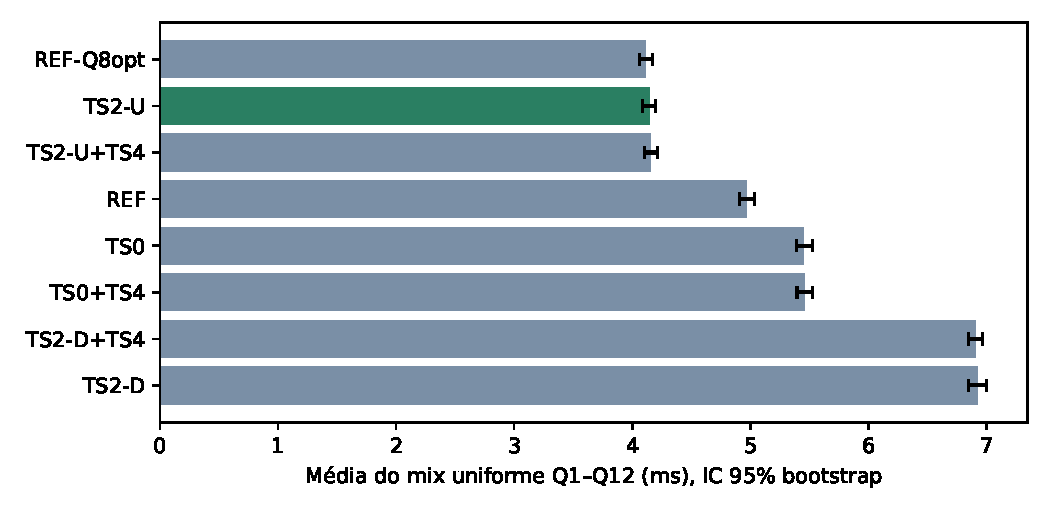
\includegraphics[width=\linewidth]{figs/iot_mix.pdf}\end{minipage}\hfill
\begin{minipage}{0.5\linewidth}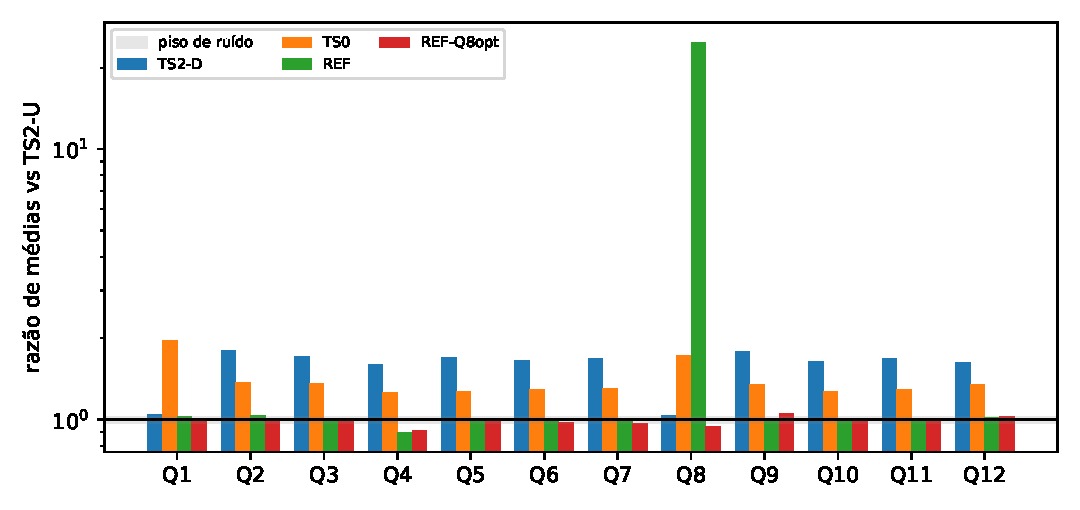
\includegraphics[width=\linewidth]{figs/iot_perquery.pdf}\end{minipage}
\caption{IoT-Benchmark. Esquerda: média do mix. Direita: razão por classe em relação a TS2-U (faixa: piso de ruído).}
\end{figure}
\paragraph{Resultados.}
\begin{itemize}
\item TS2-U, o rank 1 do seletor, é o melhor medido e empata com REF-Q8opt (razão 1,007), o que é esperado para o mesmo DDL.
\item TS0 é 1,32$\times$ mais lento e TS2-D 1,67$\times$ (piso de ruído de 2,2\%). O \emph{bucket} diário custa uma chamada CQL por dia da janela.
\item TS0 ocupa 1,8$\times$ o disco e leva 2,2$\times$ o tempo de carga. A fronteira de Pareto medida em três objetivos tem um único ponto, TS2-U, que o HBench contém.
\item Previsão estrutural: as chamadas e as linhas previstas pelo Stage 7 coincidiram com as observadas em 72/72 rotas.
\item Ablações: só a neutralização de TS2 ou de M1 piora o HBench (regret de 31,6\%); 8 regras não ativam nesta carga.
\item A REF original só perde no Q8 (24,9$\times$), por usar varredura completa em vez de leitura descendente.
\end{itemize}

\subsection{TPCx-IoT}
\paragraph{Workload e dados.} Uma adaptação de pesquisa, não oficial, do TPCx-IoT v2.1.2. Os eventos seguem o registro lógico do TPC (estação, sensor, timestamp, leitura e 900\,B de \emph{padding}) e são gerados de forma determinística: 2 subestações $\times$ 3 sensores, 130 passos de semente e 500 passos medidos, ou seja, \textbf{3.780 eventos por execução}. A carga é ingestão concorrente: um writer insere passo a passo, e 2 threads fazem 120 leituras de duas janelas de 5\,s (uma recente e uma histórica) em checkpoints selados, filtradas só por \texttt{sensor\_name}.

\paragraph{Fase de projeto.} Ativam-se TS0, TS1 e TS3, com M1 e M3. Os candidatos são \texttt{ts0\_series\_raw}, \texttt{ts1\_series\_\{3600s,60s\}} e \texttt{ts3\_sensor\_\{3600s,60s\}}. São \textbf{9 coberturas admissíveis}: uma fonte canônica e no máximo uma projeção TS3. O escore usa pesos de 45/15/20/15/5 sobre 5 proxies estruturais, normalizados pelo controle TS0. O HBench tem 5 deployments, com o controle TS0 obrigatório e diversidade de tabelas.

\paragraph{Medição.} 12 variantes: 9 admissíveis, o baseline lógico TPC (uma tabela particionada por \texttt{sensor\_name}) e réplicas A/A explícitas do rank 1 e do baseline, porque não há pares naturais. Foram 5 repetições a frio com ordem contrabalançada e keyspace novo em cada execução, totalizando 60 execuções. Todas passaram pela auditoria integral de todos os registros após a ingestão.

\begin{table}[H]\centering\footnotesize
\caption{TPCx-IoT (4.1.12): leitura sob ingestão concorrente (ms), requisições CQL por leitura, ingestão (eventos/s) e disco (KiB).}
\resizebox{\linewidth}{!}{\begin{tabular}{@{}llrcrcrr@{}}\toprule
Variante & Papel & Média & IC 95\% & p95 & CQL & ev/s & KiB\\\midrule
\tabin{tables/tpcx_summary.tex}
\bottomrule\end{tabular}}\end{table}
\begin{figure}[H]\centering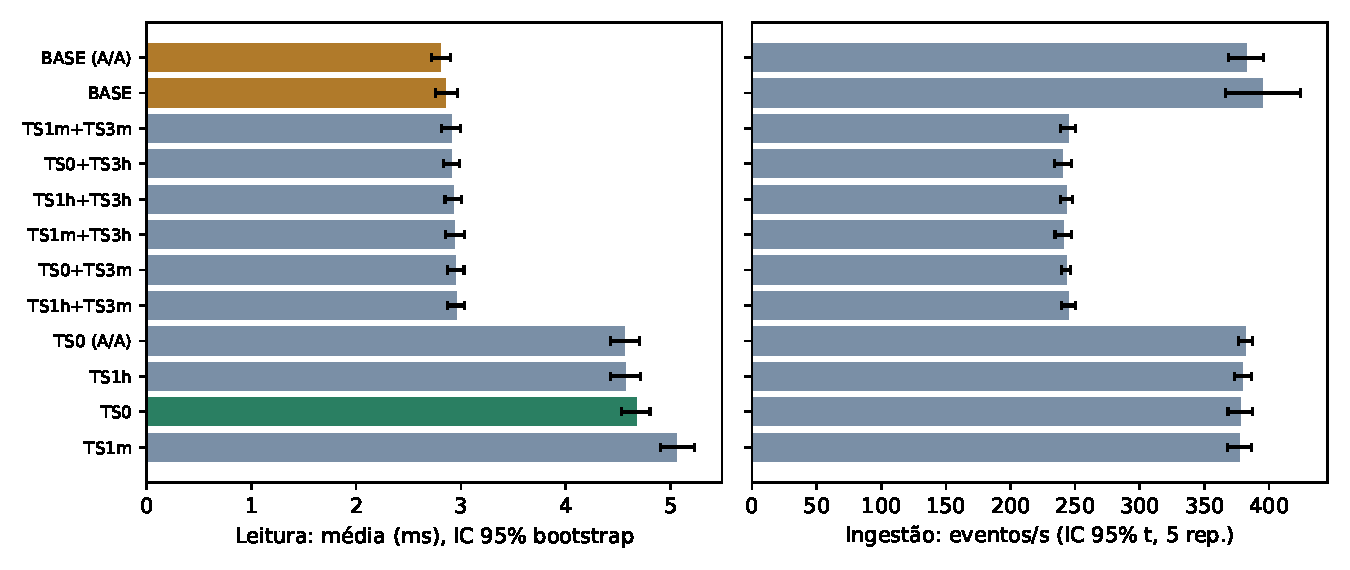
\includegraphics[width=0.85\linewidth]{figs/tpcx.pdf}\caption{TPCx-IoT: leitura (IC bootstrap) e ingestão (IC $t$).}\end{figure}
\paragraph{Resultados.}
\begin{itemize}
\item Ler de uma projeção TS3 (2--3 requisições CQL) é $\approx$37\% mais rápido que ler de TS0/TS1 (4--6 requisições). Os seis deployments com TS3 empatam entre si.
\item O custo é escrever cada evento duas vezes: a ingestão cai $\approx$36\% (243 contra 380\,ev/s) e o disco dobra.
\item O HBench contém o melhor medido (regret 0) e retém 100\% do Pareto 2D (leitura, ingestão) e 83\% do 3D.
\item O escore do seletor, porém, não ordena a leitura ($\tau=-0{,}06$; ele aponta o controle TS0): a preservação vem da salvaguarda de diversidade.
\item O \textbf{baseline lógico TPC empata em leitura com os melhores deployments, ingere 1,6$\times$ mais rápido que eles e ocupa metade do disco}. É exatamente o desenho ``TS3 como fonte canônica'', que o catálogo proíbe.
\item Ablação: só a neutralização de TS3 degrada o HBench (regret de 57\%).
\end{itemize}

\subsection{TSBS (cpu-only)}
\paragraph{Workload e dados.} O gerador oficial \texttt{tsbs\_generate\_data}, no commit \texttt{8323e59c}, foi compilado num container \texttt{golang:1.22.5} descartável. Configuração: \texttt{cpu-only}, 40 hosts, intervalo de 600\,s, 36\,h, ou seja, \textbf{8.640 observações $\times$ 10 métricas = 86.400 células}. No commit fixado, o gerador emite \texttt{series\_bigint}, e um adaptador sem perda converte o tipo para o loader do Stage 9. Os 16 templates do TSBS são: \texttt{single-groupby} (6 variantes), \texttt{cpu-max-all} (1, 8 e 32 hosts $\times$ 24\,h), \texttt{double-groupby} (1, 5 e todas as métricas), \texttt{high-cpu} (1 e todos), \texttt{lastpoint} e \texttt{groupby-orderby-limit}. Foram geradas 3 instâncias por template em duas coortes, totalizando 96: \emph{natural} (janelas arbitrárias, como o TSBS gera; métrica de decisão) e \emph{aligned} (janelas alinhadas, premissa do perfil condicional).

\paragraph{Fase de projeto.} Ativam-se TS0 (16 templates), TS5 (13), TS6 (3), TS1 (2) e TS2 (1); M1 e M3. São 9 candidatos físicos. O espaço tem dois perfis: \texttt{conservative} (2 coberturas, sem \emph{rollups}) e \texttt{conditional\_aligned} (24 coberturas). O Pareto analítico tem 2 + 8 deployments e o HBench, 2 + 5 = 7. Com 26 admissíveis, mais que 12, o protocolo exige o HBench mais o baseline; acrescentaram-se os 3 deployments do Pareto cortados pelo top-$k$.

\paragraph{Medição.} 12 variantes, entre elas o esquema Cassandra original do TSBS (\texttt{series\_bigint}, partição por série e dia) e uma réplica A/A. Um \textbf{oráculo independente} implementa os 16 templates sobre os eventos-fonte; foi validado em 960/960 respostas antes de medir. Desvio declarado: 12 rodadas por repetição em vez de 60, ou seja, 60 amostras por classe e variante no total, porque cada rodada executa 384 consultas pesadas.

\begin{table}[H]\centering\footnotesize
\caption{TSBS (4.1.12): média do mix dos 16 templates (ms) nas coortes natural e aligned, instâncias em fallback TS0 (de 96), disco e carga.}
\resizebox{\linewidth}{!}{\begin{tabular}{@{}llrcrcrrr@{}}\toprule
Variante & Papel & Natural & IC 95\% & Aligned & IC 95\% & FB & KiB & Carga (s)\\\midrule
\tabin{tables/tsbs_summary.tex}
\bottomrule\end{tabular}}\end{table}
\begin{figure}[H]\centering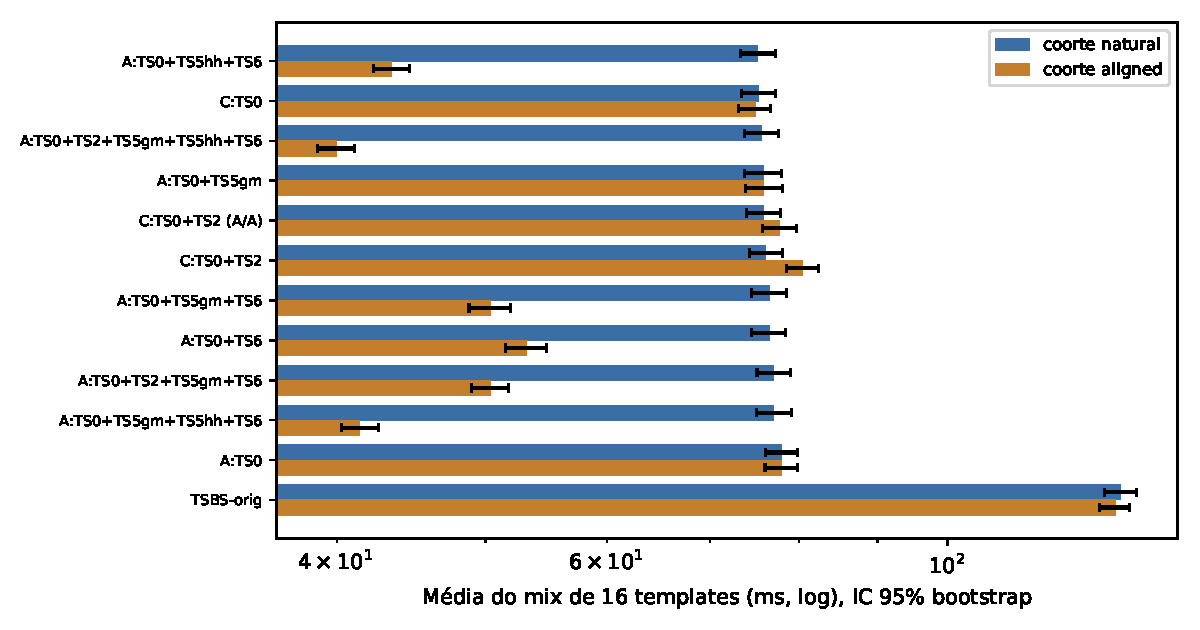
\includegraphics[width=0.8\linewidth]{figs/tsbs.pdf}\caption{TSBS: média do mix por coorte (escala log). C: perfil conservative; A: conditional\_aligned.}\end{figure}
\paragraph{Resultados.}
\begin{itemize}
\item \textbf{Coorte natural.} Todos os deployments do SchemaLens empatam ($\approx$75--78\,ms; piso de 3,4\%) e são \textbf{1,70$\times$ mais rápidos que o esquema original do TSBS} (IC [1,65; 1,76]). Parte do ganho vem do plano de leitura: \texttt{lastpoint} é 8$\times$ mais rápido com leitura descendente por (host, métrica).
\item \textbf{Coorte aligned.} Os \emph{rollups} TS5/TS6 reduzem a média a 0,50--0,66 do conservative rank 1. Os melhores são os HBench \#2 e \#4 (regret 0; $\tau=0{,}54$).
\item Com janelas arbitrárias, as rotas condicionais caem em TS0 (3--21 de 48 instâncias) e o ganho desaparece. O perfil condicional depende de uma premissa que o gerador TSBS não garante.
\item Ablações: TS6 e TS5 são as regras decisivas na coorte aligned (regret de até 0,88 e 0,33); sem TS0, o pipeline é inviável.
\end{itemize}

\subsection{Avaliação do método nos TSDB}
\begin{table}[H]\centering\small
\caption{Preservação e ordenação no espaço medido. Top-1: o rank 1 do seletor empata com o melhor medido (no TPCx o rank 1 é o controle obrigatório, não uma previsão). Piso: piso de ruído A/A da métrica de decisão.}
\begin{tabular}{@{}lrrcrrrr@{}}\toprule
Benchmark & Espaço & HBench & Top-1 & Regret & Retenção de Pareto & $\tau$ & Piso\\\midrule
\tabin{tables/method_eval.tex}
\bottomrule\end{tabular}\end{table}

% =====================================================================
\section{Experimento RUBiS}\label{sec:rubis}
% =====================================================================
\subsection{Workload, fase de projeto e restrição de dados}
O RUBiS (leilões) é modelado em EER com 7 entidades e 10 relacionamentos, e o workload \texttt{rubis.rb} tem 36 instruções e 4 cargas: Browsing, Bidding, Update10x e Update100x. A V9 do SchemaLens ativa C0--C9 por predicados quantitativos sobre estatísticas observadas, gera $P=57$ especificações, canonicaliza e funde para $C=24$ tabelas, sintetiza rotas por código, calibra o modelo de custo e seleciona \textbf{$H$ = 5 esquemas} (H01--H05) por ILP. Os baselines são NoSE~\cite{nose} e QPG, reconstruídos, mais o V8\_AUTO\_H\_norm. Essa fase foi congelada (hash \texttt{8446365297fc4918\ldots}) e não foi alterada.

A V9 original mediu em Cassandra 3.11.11, sobre um \texttt{rubis\_full} de \textbf{70,4 M linhas} (13 tabelas; 2 M itens, 20 M lances, 10 M comentários, 2 M buynow, 200 mil usuários). Esse banco existe só na máquina original e foi gerado sem semente.

\subsection{Regeneração da fonte}
Reconstruímos a fonte de forma determinística (semente 20261117):
\begin{itemize}
\item \textbf{Estrutura modular}: vem dos fan-outs exatos do E04 da V9 (10 itens por vendedor, 4.000 itens por categoria, 4.000 usuários por região, 500 pares região $\times$ categoria, 10 lances por item, 100 por usuário, 50 comentários enviados e recebidos por usuário) e das convenções do código da V8 (itens do vendedor $u$ = $u+k\cdot 200000$).
\item \textbf{Valores}: contrato do \texttt{fake.js} do NoSE.
\item \textbf{Datas crescentes com o id}: inferidas do fato de que o NoSE, que ordena por id, concordava 100\% com o contrato, que ordena por data.
\item \textbf{Coorte}: as 5 primeiras páginas de 1.000 linhas por ordem de token Murmur3 $\cup$ o fecho do domínio do benchmark, pela regra da V8.
\end{itemize}
Resultado: 7.392 itens, 7.083 usuários (21.855 no fecho), \textbf{5.690 lances e 5.300 buynow, idênticos à V9}, 6.529 comentários (6.501 na V9), 500 categorias e 50 regiões.

\subsection{Medição em duas versões}
Os mesmos dados foram carregados em dois nós dedicados, \textbf{4.1.12 e 3.11.11}, com hashes idênticos das funções da V9 nos dois. Foram medidos 9 deployments (H01--H05, NoSE, QPG, V8\_AUTO\_H\_norm e a réplica A/A H01\_AA). O protocolo de requisições é o da V9: 4 cargas $\times$ (1.000 aquecimentos + 10.000 medidas), histórias semeadas e restauração de estado. Foram 5 repetições a frio, com as versões intercaladas em ABBA e só um nó ligado por vez. A corretude é conferida pelo \textbf{oráculo independente da V9} (contrato E6 das 36 instruções): \textbf{3.577.311 instruções por versão, 100\% de concordância}.

\begin{table}[H]\centering\scriptsize
\caption{RUBiS em Cassandra 4.1.12: média por requisição (ms) e IC 95\% bootstrap pareado.}
\begin{tabular}{@{}lcccc@{}}\toprule
Deployment & Browsing & Bidding & Update10x & Update100x\\\midrule
\tabin{tables/rubis_mean_v41.tex}
\bottomrule\end{tabular}\end{table}
\begin{table}[H]\centering\scriptsize
\caption{RUBiS em Cassandra 3.11.11 (mesmos dados): média por requisição (ms) e IC 95\%.}
\begin{tabular}{@{}lcccc@{}}\toprule
Deployment & Browsing & Bidding & Update10x & Update100x\\\midrule
\tabin{tables/rubis_mean_v311.tex}
\bottomrule\end{tabular}\end{table}
\begin{figure}[H]\centering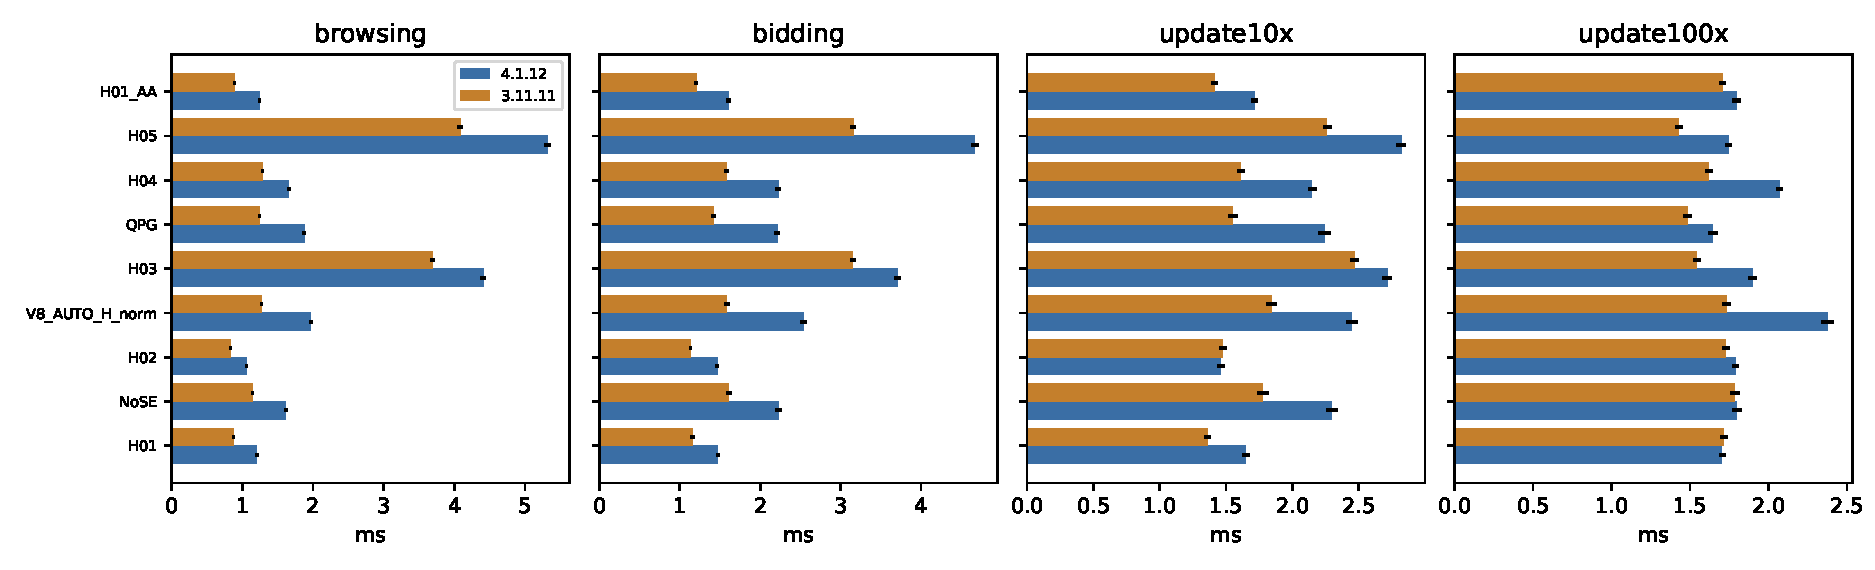
\includegraphics[width=\linewidth]{figs/rubis.pdf}\caption{RUBiS: média por carga em 4.1.12 e 3.11.11, com os mesmos dados e o mesmo protocolo.}\end{figure}
\begin{table}[H]\centering\scriptsize
\caption{RUBiS: razão H/baseline em 4.1.12 / 3.11.11. \textbf{H+}: H mais rápido; H$-$: mais lento.}
\begin{tabular}{@{}llcccc@{}}\toprule
H & Baseline & Browsing & Bidding & Update10x & Update100x\\\midrule
\tabin{tables/rubis_contrasts.tex}
\bottomrule\end{tabular}\end{table}
\begin{table}[H]\centering\small
\caption{RUBiS: efeito da versão e ordenação do modelo de custo.}
\begin{tabular}{@{}lcccc@{}}\toprule
 & Browsing & Bidding & Update10x & Update100x\\\midrule
\tabin{tables/rubis_version.tex}
\bottomrule\end{tabular}\end{table}
\paragraph{Resultados.}
\begin{itemize}
\item \textbf{A conclusão da V9 se replica.} Em 4.1.12, H01 é 25--36\% mais rápido que NoSE e QPG em browsing, bidding e update10x; em update100x empata. O mesmo vale em 3.11.11, e era o resultado da V9 original.
\item \textbf{Modelo de custo.} Ele ordena H corretamente em browsing e bidding ($\tau$ de 0,95 a 1,00) e razoavelmente em update10x (0,80). Falha em update100x ($\tau$ de 0,20 a 0,40), carga em que os cinco esquemas ficam a menos de 25\% uns dos outros.
\item \textbf{Efeito da versão.} Com os mesmos dados, o 4.1.12 é 1,14--1,38$\times$ mais lento (média geométrica por carga). As ordenações se preservam onde as diferenças são grandes ($\tau$ entre versões de 0,78 a 0,94) e se embaralham em update100x ($\tau=0{,}28$). Dos 60 vereditos H $\times$ baseline, 46 são iguais nas duas versões.
\item \textbf{Hipóteses.} H1 (H01 supera os baselines) e H5 (corretude total) foram confirmadas. H2--H4 foram rejeitadas, todas por update100x.
\end{itemize}

% =====================================================================
\section{Aceitação}
% =====================================================================
\begin{table}[H]\centering\small
\caption{Gates recalculados dos dados brutos, testes negativos, janelas descartadas e hipóteses pré-registradas ($\checkmark$ confirmada, $\times$ rejeitada).}
\begin{tabular}{@{}lccc l@{}}\toprule
Benchmark & Gates & Testes negativos & Janelas descartadas & Hipóteses H1--H5\\\midrule
\tabin{tables/acceptance.tex}
\bottomrule\end{tabular}\end{table}

% =====================================================================
\section{Discussão}
% =====================================================================
\paragraph{O que a metodologia demonstra.} Nos três TSDB, a redução explicável preservou o melhor deployment medido (regret de 0--0,2\%) com redução de 44--50\% do espaço, e cada exclusão tem uma razão registrada: regra não ativada, guard inelegível, dominância ou corte de top-$k$. As ablações mostram quais regras sustentam a decisão em cada carga: TS2/M1 no IoT, TS3 no TPCx, TS5/TS6 no TSBS alinhado. Mostram também que regras não ativadas não têm efeito, o que é coerente com a explicabilidade.

\paragraph{O que ela não demonstra.} (i) O escore analítico só ordena bem a latência quando há diferenças estruturais grandes: $\tau$ = 0,87 no IoT, mas $-$0,06 no TPCx e $-$0,09 no TSBS natural, onde a preservação vem da salvaguarda de diversidade. (ii) Ganho sobre o desenho de referência é condicional à carga: nenhum no IoT (mesmo DDL), empate em leitura e perda em escrita no TPCx, ganho de 1,7$\times$ no TSBS e de 25--36\% no RUBiS diante de NoSE/QPG. (iii) No TPCx, o catálogo exclui o melhor desenho global (TS3 como fonte canônica), o que é uma limitação do espaço de candidatos.

\paragraph{Versão do Cassandra.} O experimento pareado do RUBiS mostra que a versão, sozinha, muda as latências absolutas em até 38\% e pode embaralhar ordenações quando as diferenças entre esquemas são pequenas. A harmonização em 4.1.12 era necessária para comparar benchmarks.

% =====================================================================
\section{Ameaças à validade}
% =====================================================================
\begin{itemize}
\item \textbf{Interna}: latência ponta a ponta no cliente Python (driver + pós-processamento); nó único, RF\,=\,1; dados pequenos o bastante para o page cache (``frio'' = JVM e caches do Cassandra). No TSBS, o desvio declarado foi de 12 rodadas por repetição.
\item \textbf{Construto}: média de mix uniforme (sem frequências oficiais); proxies estruturais calculados na escala modelada, não na executada (TPCx); armazenamento após flush, sem compactação de longo prazo.
\item \textbf{Externa}: escalas de piloto nos TSDB (54 mil, 3.780 por execução e 86.400 células); TPCx-IoT não oficial; no RUBiS, dados regenerados (estrutura reconstruída, não o \texttt{rubis\_full} original) e sem escala completa (E23).
\item \textbf{Conclusão}: desenvolvimento iterativo das versões do seletor, mitigado por congelamento, pré-registro e hipóteses rejeitadas mantidas como resultado.
\end{itemize}

% =====================================================================
\section{Conclusão}
% =====================================================================
O SchemaLens produz, antes de medir, um conjunto pequeno e auditável de projetos físicos completos para o Cassandra. Sob um protocolo comum de execução, com a mesma versão, as mesmas métricas, a mesma estatística, o mesmo controle físico e corretude por oráculo em todas as respostas, essa redução preservou os melhores deployments nos três benchmarks de séries temporais. Também confirmou, no RUBiS e com dados regenerados, a vantagem dos esquemas gerados sobre NoSE e QPG nas cargas de leitura e mistas. As limitações encontradas (escore pouco preditivo da latência em espaços com empates, espaço de candidatos que exclui o baseline TPCx e dependência de premissas de alinhamento no TSBS) indicam onde a metodologia deve evoluir.

\begin{thebibliography}{99}\small
\bibitem{lakshman} A.~Lakshman, P.~Malik. Cassandra: a decentralized structured storage system. \emph{ACM SIGOPS OSR}, 44(2), 2010.
\bibitem{chebotko} A.~Chebotko, A.~Kashlev, S.~Lu. A Big Data Modeling Methodology for Apache Cassandra. \emph{IEEE BigData Congress}, 2015.
\bibitem{nose} M.~J.~Mior, K.~Salem, A.~Aboulnaga, R.~Liu. NoSE: Schema Design for NoSQL Applications. \emph{IEEE ICDE}, 2016.
\bibitem{modelardb} S.~K.~Jensen, T.~B.~Pedersen, C.~Thomsen. ModelarDB: Modular Model-Based Time Series Management with Spark and Cassandra. \emph{PVLDB}, 11(11), 2018.
\bibitem{iotbench} R.~Liu, J.~Yuan et al. Benchmarking Time Series Databases with IoTDB-Benchmark for IoT Scenarios. arXiv:1901.08304, 2019.
\bibitem{tpcx} Transaction Processing Performance Council. TPCx-IoT Standard Specification v2.1.2.
\bibitem{tsbs} Timescale. Time Series Benchmark Suite (TSBS). \url{https://github.com/timescale/tsbs}.
\bibitem{rubis} E.~Cecchet et al. Performance and Scalability of EJB Applications. \emph{OOPSLA}, 2002 (RUBiS).
\bibitem{ehrgott} M.~Ehrgott. \emph{Multicriteria Optimization}. Springer, 2005.
\bibitem{efron} B.~Efron, R.~J.~Tibshirani. \emph{An Introduction to the Bootstrap}. Chapman \& Hall, 1993.
\bibitem{hyndman} R.~J.~Hyndman, Y.~Fan. Sample quantiles in statistical packages. \emph{The American Statistician}, 50(4), 1996.
\bibitem{nosek} B.~A.~Nosek et al. The preregistration revolution. \emph{PNAS}, 115(11), 2018.
\end{thebibliography}
\end{document}
